    \section{Vista de Casos de Uso} \label{vistaCasosDeUso}
    En esta vista se describirá el sistema desde el punto de vista de los casos de uso. El sistema tiene 2 actores:

    \begin{itemize}
        \item \emph{Admin}: Administrador de CPI. Es un usuario de Umbraco, lo que quiere decir que cuenta con las credenciales para poder ingresar al back-end de Umbraco y tiene los permisos necesarios para administrar las entidades y los grupos de CPI.
        \item \emph{cpi-user}: Es un grupo de CPI, los pertenecientes a este grupo poseen credenciales para entrar al sistema.
        \item \emph{Retailer}: Representa a una cadena. Solo tiene acceso a la información referente a las tiendas y productos que pertenecen a la cadena.
         \end{itemize}

    \subsection{Resumen de Casos de Uso}
    \newcounter{magicrownumbers}
    \newcommand\rownumber{\stepcounter{magicrownumbers}\arabic{magicrownumbers}}
    \begin{center}
        \begin{longtable}{ | l | l | c | }
            \hline
            \rowcolor{blue!25}
            \multicolumn{1}{|c|}{ID del Caso de Uso} &
            \multicolumn{1}{|c|}{Caso de Uso} &
            \multicolumn{1}{|c|}{Actor} \\
            \hhline{===}
            \endhead

            \endfoot

           CU-\rownumber & Iniciar sesión (Umbraco) & Admin \\ \hline
           CU-\rownumber & Consultar lista miembros & Admin \\ \hline
           CU-\rownumber & Gestionar miembro (CRUD) & Admin \\ \hline
           CU-\rownumber & Consultar grupos & Admin \\ \hline
           CU-\rownumber & Gestionar grupo (CRUD) & Admin \\ \hline
           CU-\rownumber & Asignar miembro/s a grupo & Admin \\ \hline
           CU-\rownumber & Remover miembro/s de grupo (CRUD) & Admin \\ \hline
           CU-\rownumber & Cambiar permisos de miembro & Admin \\ \hline

           CU-\rownumber & Gestionar contenido & Admin \\ \hline
           CU-\rownumber & Consultar lista de cadenas & Admin \\ \hline
           CU-\rownumber & Gestionar cadena (CRUD) & Admin \\ \hline
           CU-\rownumber & Consultar lista de productos & Admin \\ \hline
           CU-\rownumber & Gestionar producto (CRUD) & Admin \\ \hline
           CU-\rownumber & Consultar lista de productos UPC & Admin \\ \hline
           CU-\rownumber & Gestionar producto UPC (CRUD) & Admin \\ \hline
           CU-\rownumber & Asignar producto/s a producto UPC & Admin \\ \hline
           CU-\rownumber & Remover producto/s de producto UPC & Admin \\ \hline
           CU-\rownumber & Consultar lista de precios & Admin \\ \hline
           CU-\rownumber & Consultar lista de tiendas & Admin \\ \hline
           CU-\rownumber & Gestionar tienda (CRUD) & Admin \\ \hline
           CU-\rownumber & Consultar lista de zonas & Admin \\ \hline
           CU-\rownumber & Gestionar zonas (CRUD) & Admin \\ \hline
	       CU-\rownumber & Consultar lista de catálogo generales & Admin \\ \hline
           CU-\rownumber & Gestionar catálogo (CRUD) & Admin \\ \hline
           CU-\rownumber & Asignar producto/s a catálogo & Admin \\ \hline
           CU-\rownumber & Remover producto/s de catálogo & Admin \\ \hline

           
           CU-\rownumber & Iniciar sesión (CPI) & Retailer \\ \hline
           CU-\rownumber & Consultar lista de productos & Retailer \\ \hline
           CU-\rownumber & Importar precios desde archivo excel & Retailer \\ \hline
           CU-\rownumber & Consultar precio producto & Retailer \\ \hline
           CU-\rownumber & Consultar histórico de producto & Retailer \\ \hline
           CU-\rownumber & Consultar gráfico dispersión por categoría & Retailer \\ \hline
           CU-\rownumber & Filtrar gráfico dispersión por categoría & Retailer \\ \hline
           CU-\rownumber & Consultar lista de catálogos personalizados & Retailer \\ \hline
           CU-\rownumber & Gestionar catálogo (CRUD) & Retailer \\ \hline
           CU-\rownumber & Asignar producto/s a catálogo & Retailer \\ \hline
           CU-\rownumber & Remover producto/s de catálogo & Retailer \\ \hline

        \end{longtable}
    \end{center}

    \subsection{Diagrama de Casos de Uso}
    Se separaron los casos de uso en varios diagramas para facilitar la lectura.

    \begin{figure}[H]
        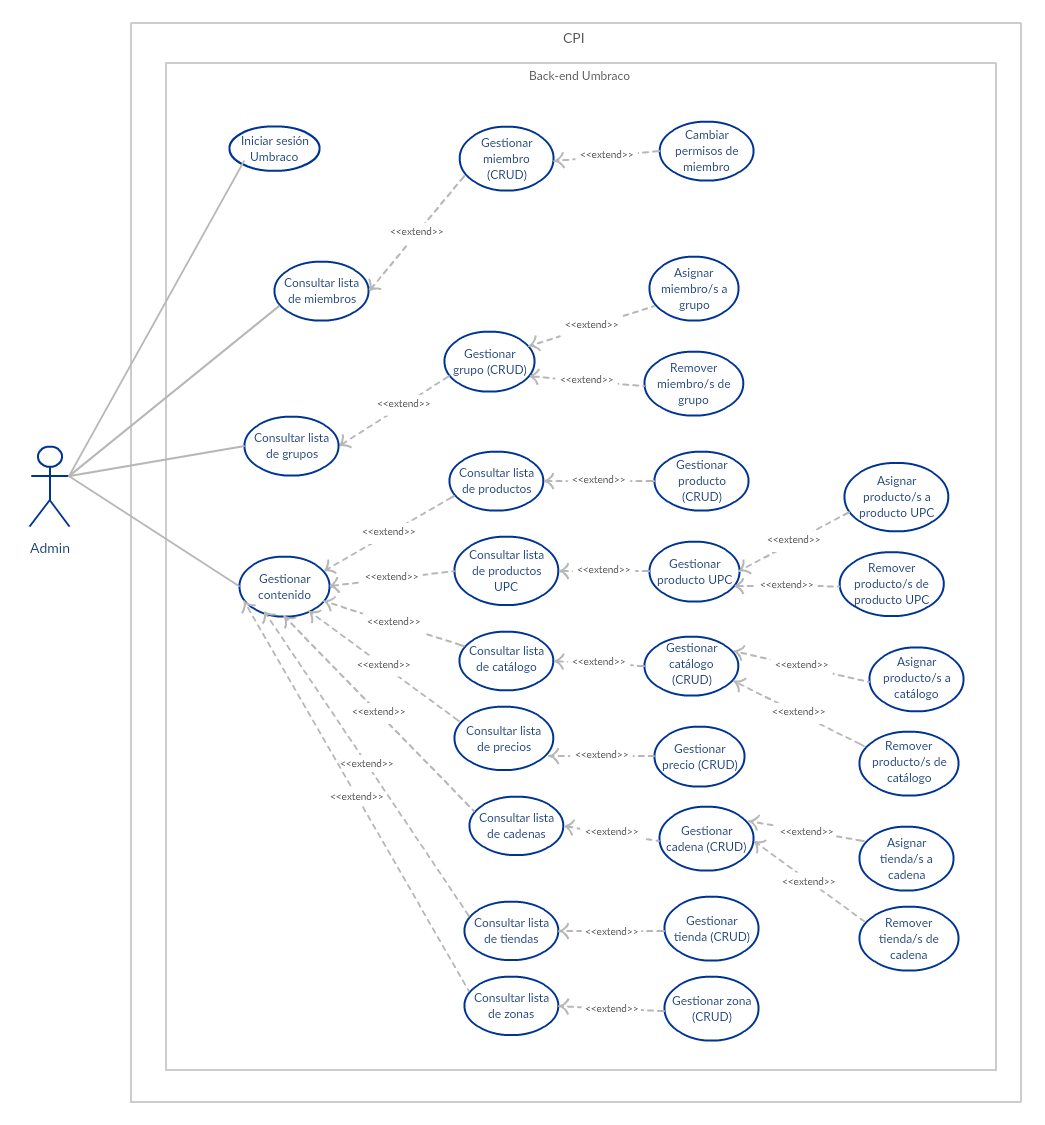
\includegraphics[width=\textwidth]{cu_admin.png}
        \caption{Casos de uso para usuario Admin}
        \label{fig:cu_admin}
        \centering
    \end{figure}

    \begin{figure}[H]
        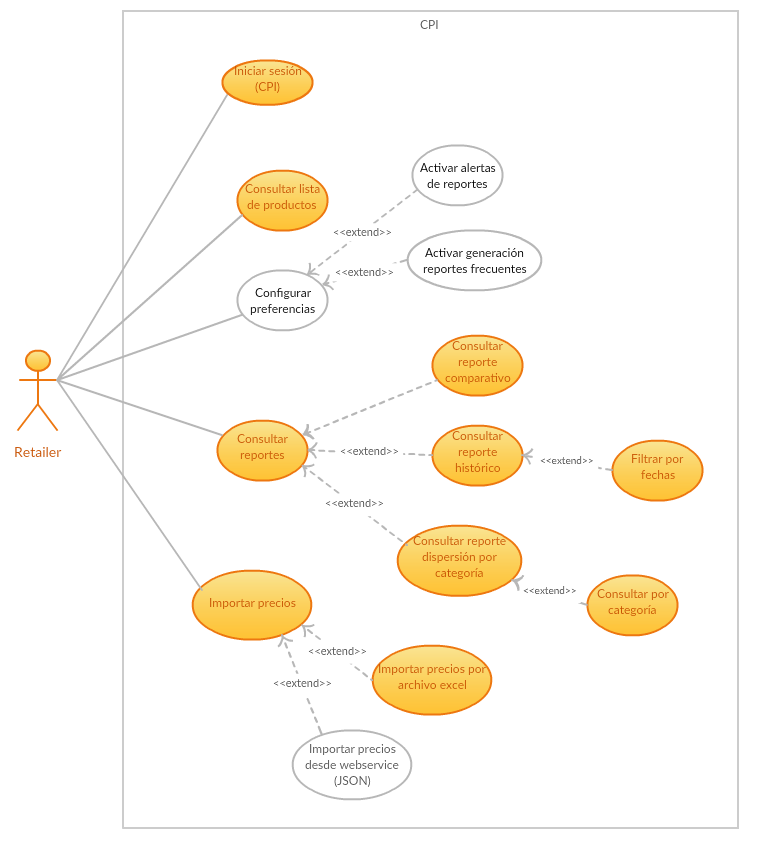
\includegraphics[scale=0.8]{cu_retailer.png}
        \caption{Casos de uso para usuario Retailer}
        \label{fig:cu_retailer}
        \centering
    \end{figure}

    \subsection{Especificaciones de Casos de Uso}
    A continuación las narrativas de los casos de uso:

    \begin{center}
        \begin{longtabu} to 0.9\textwidth { | X[p] | X[p] | }
            \hline
            \multicolumn{2}{|l|}{
                \cellcolor{blue!25}{\large{\textbf{Caso de Uso:}} Iniciar sesión (Umbraco)}
            } \TBstrut \\
            \hline\hline

            \multicolumn{2}{|l|}{
                \makecell{\large{\textbf{Descripción:}} \\ El usuario quiere ingresar al back end de Umbraco.}
            } \\
            \hline

            \multicolumn{2}{|l|}{
                \makecell{\large{\textbf{Precondición:}} \\ Ingresar la dirección correcta del sitio en la barra de navegación.}
            } \\
            \hline


            \multicolumn{2}{|l|}{\cellcolor{blue!15}\large{\textbf{Flujo básico:}}}  \TBstrut\\
            \hline

            Actor & Sistema \TBstrut\\
            \hline
            1. El actor abre su navegador e introduce la dirección correspondiente al back end de Umbraco. &  \\ [0.3ex]
            \hline
             & 2. El servidor procesa la solicitud y envía al navegador del cliente una ventana para que el usuario se autentique. \\ [0.3ex]
             \hline
             3. El actor introduce su email y su contraseña. &  \\ [0.3ex]
             \hline
             & 4. El sistema valida la información del usuario y lo redirige al tablero (back end) de Umbraco. \\ [0.3ex]
             \hline\hline


            \multicolumn{2}{|l|}{\cellcolor{blue!15}\large{\textbf{Flujos alternos:}}}  \TBstrut\\
            \hline

            Actor & Sistema \TBstrut\\
            \hline
            1. El actor abre su navegador e introduce la dirección correspondiente al back end de Umbraco. &  \\ [0.3ex]
            \hline
             & 2. El servidor procesa la solicitud y envía al navegador del cliente una ventana para que el usuario se autentique. \\ [0.3ex]
             \hline
             3. El actor introduce su email y su contraseña. &  \\ [0.3ex]
             \hline
             & 4. El sistema no valida la información del usuario y lo redirige a la misma página de inicio de sesión indicándole que los datos introducidos son incorrectos. \\ [0.3ex]
             \hline\hline

            \multicolumn{2}{|l|}{
                \makecell{\large{\textbf{Poscondición:}} \\ El usuario se encuentra en el tablero de Umbraco.}
            } \\
            \hline
            \multicolumn{2}{|l|}{
                \makecell{\large{\textbf{Puntos de extensión:}} \\ No se requiere de otros casos de uso.}
            } \\
            \hline
        \end{longtabu}
    \end{center}
    \vspace{-4em}

    \begin{center}
        \begin{longtabu} to 0.9\textwidth { | X[p] | X[p] | }
            \hline
            \multicolumn{2}{|l|}{
                \cellcolor{blue!25}{\large{\textbf{Caso de Uso:}} Consultar lista de miembros}
            } \TBstrut \\
            \hline\hline
            \multicolumn{2}{|l|}{
                \makecell{\large{\textbf{Descripción:}} \\ El usuario quiere consultar la lista de miembros de CPI.}
            } \\
            \hline
            \multicolumn{2}{|l|}{
                \makecell{\large{\textbf{Precondición:}} \\ Haber ingresado al back end de Umbraco.}
            } \\
            \hline
            \multicolumn{2}{|l|}{\cellcolor{blue!15}\large{\textbf{Flujo básico:}}}  \TBstrut\\
            \hline

            Actor & Sistema \TBstrut\\
            \hline
            1. El usuario le da click a la sección "Members" en el tablero de Umbraco. &  \TBstrut\\
            \hline
            & 2. El sistema muestra el panel de miembros. \TBstrut\\
            \hline
            3. El usuario le da click a la carpeta "Members". &  \TBstrut\\
            \hline
            & 4. El sistema muestra la lista de los miembros de CPI. \TBstrut\\
            \hline\hline


            \multicolumn{2}{|l|}{\cellcolor{blue!15}\large{\textbf{Flujos alternos:}}}  \TBstrut\\
            \hline
            Actor & Sistema \TBstrut\\
            \hline
            1. El actor hace algo. &  \TBstrut\\
            \hline
             & 2. El sistema responde. \TBstrut\\
             \hline\hline


            \multicolumn{2}{|l|}{
                \makecell{\large{\textbf{Poscondición:}} \\ Aquí va la poscondición del caso de uso.}
            } \\
            \hline
            \multicolumn{2}{|l|}{
                \makecell{\large{\textbf{Puntos de extensión:}} \\ Aquí van los puntos de extensión del caso de uso.}
            } \\
            \hline
        \end{longtabu}
    \end{center}
    \vspace{-4em}

    \begin{center}
        \begin{longtabu} to 0.9\textwidth { | X[p] | X[p] | }
            \hline
            \multicolumn{2}{|l|}{
                \cellcolor{blue!25}{\large{\textbf{Caso de Uso:}} Nombre del caso de uso}
            } \TBstrut \\
            \hline\hline
            \multicolumn{2}{|l|}{
                \makecell{\large{\textbf{Descripción:}} \\ Descripción del caso de uso.}
            } \\
            \hline
            \multicolumn{2}{|l|}{
                \makecell{\large{\textbf{Precondición:}} \\ Aquí va la precondición.}
            } \\
            \hline
            \multicolumn{2}{|l|}{\cellcolor{blue!15}\large{\textbf{Flujo básico:}}}  \TBstrut\\
            \hline

            Actor & Sistema \TBstrut\\
            \hline
            1. El actor hace algo. &  \TBstrut\\
            \hline
             & 2. El sistema responde. \TBstrut\\
             \hline\hline


            \multicolumn{2}{|l|}{\cellcolor{blue!15}\large{\textbf{Flujos alternos:}}}  \TBstrut\\
            \hline
            Actor & Sistema \TBstrut\\
            \hline
            1. El actor hace algo. &  \TBstrut\\
            \hline
             & 2. El sistema responde. \TBstrut\\
             \hline\hline


            \multicolumn{2}{|l|}{
                \makecell{\large{\textbf{Poscondición:}} \\ Aquí va la poscondición del caso de uso.}
            } \\
            \hline
            \multicolumn{2}{|l|}{
                \makecell{\large{\textbf{Puntos de extensión:}} \\ Aquí van los puntos de extensión del caso de uso.}
            } \\
            \hline
        \end{longtabu}
    \end{center}
    \vspace{-4em}